\chapter{Results}
\label{RESULTS}
In related studies, attempts were made to bring programming and teaching together through writing sound (cf. Sonic Pi \cite{Aaron2016Art}) or writing music (cf. Scalala). But all projects lack language fluency and assessibility. The primary purpose of this work was to create a domain-specific language to write music notation in an intuitive environment. The language was designed for novices in programming and novices in music. It is known from the literature that novices are seeking fluency to link programming constructs with natural language.\cite{Bonar1985}

To create such an environment, this thesis utilised the Scala parser combinators to define, implement and provide an external DSL library—Scalala—which converts an input DSL script into MIDI sequences. To provide an interactive user environment, a web-application, based on Scala Akka as server and Scala.js as client, was implemented. The application was forked from ScalaKata2, modified and released as ScalalaKata. As already outlined in chapter \ref{INTRO} only the combination of both yield the desired holistic application.

To reach this particular requirement, the DSL was developed as a stand-alone library and finally included as a dependency to the web application. Sbt dependency's and deployment management was used to publish Scalala and integrate it into ScalalaKata.

In this section, the results are presented in three main parts:

\begin{itemize}
\item Examining the designed language and reviewing fluency as well as usability.
\item Discussing the implemented web-approach and examining its accessibility.
\item Introducing a minor case study and discussing the results.
\end{itemize}

\section{Exploration of the DSL}
\label{RESULTS_DSL}
All following DSL script listings are illustrations from the final user interface ScalalaKata. As an overall result, figure \ref{IMG_SCREEN_M} presents an DSL script example.

The result demonstrates the definition and usage of one simple \texttt{musician} variable which holds an \texttt{instrument} and simple \texttt{notes}. Analysing the language regarding its fluency, the language strongly matches the analogy to plain English and meets the observations from Soloway.\cite{Soloway1982} If one statement is \textit{spoken} as a whole sentence, the correlation to plain English is already recognisable.

One of the aims of this thesis was to teach the fundamental programming concepts. The scope of the designed language and the provided programming principles are listed in table \ref{TBL_DSL_TEACHING}.

\begin{table}[h]
\caption{DSL notation and programming concepts.}
\label{TBL_DSL_TEACHING}
\begin{tabular}{p{200pt}|p{180pt}}
\rowcolor{htwg-teal} 
\textbf{DSL Notation}                  			& \textbf{Programming Concept}     \\
\texttt{note.[flat | sharp | dot]}            & Method invocation \\
\texttt{musician [var]}                   		& Variable declaration and usage \\
\texttt{[++ | - -]note}                    			& Prefix notation \\
\texttt{note / [2 | 4 | 8 | 16]}                 & Arithmetic \\
\texttt{musician [var1]}\newline\texttt{musician [varN]}\newline\texttt{play [var1] [varN]}		& Sequential programming \\
\texttt{chord([notes])}\newline\texttt{loop([notes])}  							& Arguments
\end{tabular}
\end{table}

Table \ref{TBL_DSL_TEACHING} also demonstrates the language cardinality related to the music cardinality. A music-domain expert should note, however, that the music notation range is not fully exploited and offers less notations than, for example, LilyPond (cf. \ref{LIT_PROJ_LILY}). Nevertheless, comprehensive music notation was not within the scope of this study, since the aim was to reduce complexity. Furthermore, the music notation represents only the metaphorical abstraction to conventional programming paradigms. For example, in table \ref{TBL_DSL_TEACHING}, \texttt{musician} is just a metaphor for the data type and variable definition in conventional programming. The metaphor approach is similar to Kahn's ToomTalkTM.\cite{Kahn1995}

Figures \ref{IMG_SCREEN_S}, \ref{IMG_SCREEN_M} and \ref{IMG_SCREEN_L} gives further examples in three complexity gradients—simple, intermediate and advanced.

\begin{figure}[h]
\caption{ScalalaKata Example \textbf{\romannumeral 1} - simple ("Twinkle, Twinkle, Little Star" - Jane Taylor)}
\label{IMG_SCREEN_S}
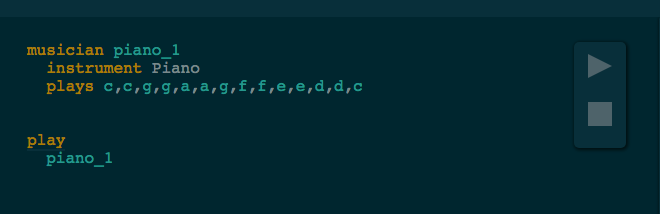
\includegraphics[scale=0.5]{screen_simple}
\end{figure}

\begin{figure}[h]
\caption{ScalalaKata Example \textbf{\romannumeral 2} - intermediate ("The Imperial March"- John Williams)}
\label{IMG_SCREEN_M}
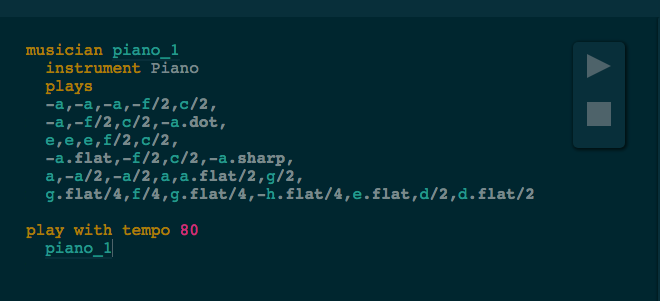
\includegraphics[scale=0.5]{screen_intermediate}
\end{figure}

\begin{figure}[h]
\caption{ScalalaKata Example \textbf{\romannumeral 3} - advanced ("Believer" - Imagine Dragons)}
\label{IMG_SCREEN_L}
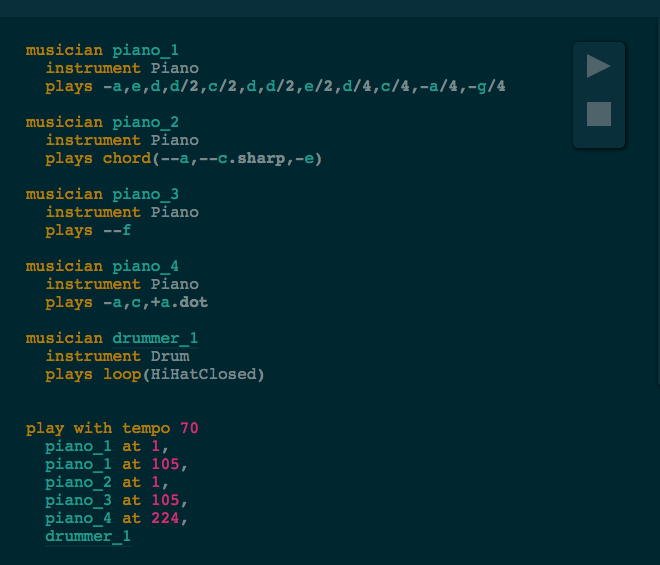
\includegraphics[scale=0.5]{screen_advanced}
\end{figure}

\paragraph{Simple}
Example \textbf{\romannumeral 1}  illustrates a DSL script in its simplest form. One \texttt{musician} and basic \texttt{notes} are used. This example already uses the concepts of variable definition and usage, lists and sequence programming. Advantages are the simplicity for both domains—programming and music novices. Disadvantages are the reduced capabilities in music composition.

\paragraph{Intermediate}
Example \textbf{\romannumeral 2} represents an intermediate implementation. In addition to example\textbf{ \romannumeral 1 }, optional parameter and method invocations were added. Advantages are higher flexibility in music and teaching of further programming concepts.

\paragraph{Advanced}
The advanced implementation, example \textbf{\romannumeral 3}, represents the entire spectrum of the language. Almost all constructs were used. As can be seen, the advanced syntax is less than perfect and may introduce some difficulties for novice programmers This complexity is in direct correlation with the music complexity.

\section{Web-Application}
\label{RESULTS_WEBAPP}
The web-application was implemented as in a cross-platform and responsive application with seamless DSL integration and Docker deployment. The usage of CodeMirror as main client library resulted in an optimal approach since CodeMirror is by default optimised for responsive applications and mobile environments.

Minor adjustments were made to provide MIDI support in cross-platform environments. By default, mobile browsers prevent playing audio through JavaScript. The user has to accept the playback and invoke the playback through an explicit interface interaction like touch gesture or click event. Because of this circumstance, in some browsers, the user has to execute the DSL script in its first instance by pressing the \texttt{play} button. After that the short-cut \texttt{Cmd + Enter} is available. Furthermore, the used \texttt{AudioContext} is not consistent across all browsers. Safari, for example, needs a different instantiation as the other engines\footnote{As of the date of publication of this thesis.}.

The web-appplication was implemented, according to the aim of this study, as an interactive solution. Compared to Sonic Pi (cf. \ref{LIT_PROJ_SONICPI}), ScalalaKata is not as interactive. In particular, Sonic Pi's advantage is a highly complex timing model, which pastes new code fragments during runtime at an calculated position, to provide a seamless transition.\cite{Aaron2014} Refer to chapter \ref{DISCUSSION} for a comprehensive discussion related to this issue.


\section{Minor Case Study}
\label{RESULTS_STUDY}
A minor case study was conducted. It should be noted, however, that this examination does not represent a complete and comprehensive case study since this is beyond the scope of this thesis. For further projects, a comprehensive study is recommended. Nevertheless, the examination revealed useful insights.

The ScalalaKata application was given to three independent users; each of them affiliated with a different domain.

\begin{itemize}
\item User A belongs to the programming domain only.
\item User B belongs to the music domain only.
\item User C belongs to the programming \textbf{and} music domain.
\end{itemize}

The users conducted the study under the same conditions:

\begin{itemize}
\item A brief introduction into the application's background was given.
\item There was no explanation in advance about syntax and usage.
\item An example DSL script was shown as an initial start script.
\item There was no defined goal. They were welcome to experiment freely.
\end{itemize}

A comprehensive table of the observed user behaviours and the report is given in appendix \ref{APPENDIX_A} and appendix \ref{APPENDIX_B}. To emphasise significant results, the following résumé relates some of the found insights to the literature.
\newline
\newline
In line with Kranch's observations, subjects from the programming domain analysed the program structure. The novice just concentrated on particular instructions and tried to derive rules from natural language to create a structure.\cite{Kranch2012} Furthermore, the programming novice named some instructions, like the \texttt{f.sharp}, by using language from the music-domain. The programming expert instead named these constructs using their programming knowledge: "I call a method of the note f". This observation is similar to Kranch's research. Kranch further mentioned that the novices "took up to three times as long as experts to analyse the short program in the study".\cite[p. 309]{Kranch2012} This observation was not met in this study: All three subjects took the same time to get familiar with the new syntax. One possible cause for this may be that the DSL language was also entirely new for the experts and they had to compare the syntax to their programming knowledge.

Beyond this, all subjects requested further guidelines regarding the syntax, since the example did not include a comprehensive syntax overview, and all subjects wanted to implement more complex music constructs. Thus, it can be concluded that the initial example script is not sufficient as a guideline. A comprehensive guidebook or more examples may be necessary.

Another interesting observation was that the programming and music expert mentioned that he/she did not compare the language to a programming language, and he/she thought just in music notation. Thus, the subject intuitively wrote  \texttt{cis} instead of thinking about method invocation. This observation supports the fluency of the DSL language and the proximity to the natural language.

Besides, all subjects stated that the error messages were not useful. In future, comprehensive exception handling and user-friendly error messages should be implemented. Chapter \ref{DISCUSSION} gives an example to improve error message handling through the Scala parser combinators.

All users had no issues with the user-interface at all. Writing the script through the provided CodeMirror instance as well as the interaction through buttons (execute/play; stop), was no problem.

\section{Performance Analysis}
\label{RESULTS_PERFOMANCE}
This paragraph concludes the result chapter with a brief performance analysis. Especially the performance of the web-application is examined since there were significant performance anomalies. Due to the small language scope and the less amount of parsers, the external DSL Scalala is negligible for the analysis.

During implementation, the web-application was mainly developed and tested with the Google Chrome browser. After completing the first prototype of the ScalalaKata application, Mozilla's Firefox browser was also tested and significant performance issues in the music playback were recognised. Further examinations revealed that the MIDI playback is extremely resource intensive. The Firefox browser is not able to playback MIDI scripts accurately if more instruments are involved and the tempo is increased over 150 bpm. The CPU load of the Google Chrome browser and Mozilla's Firefox are compared in figure \ref{IMG_CPU_BROWSER}. As can be seen for Firefox, one CPU core is continuously at 100\% load, since the CPU scheduler switches the process from core to core. However, Firefox is based on the same \texttt{AudioContext} as the Google Chrome browser; it has not been possible to provide a definite answer to this circumstance. Nevertheless, basic MIDI scripts are possible, and all other state-of-the-art browsers, including mobile-browsers, are working without any performance issues.

\begin{figure}[h]
\caption{CPU load during the ScalalaKata app running and sound playing. (Test Setup: 4 Core CPU)}
\label{IMG_CPU_BROWSER}
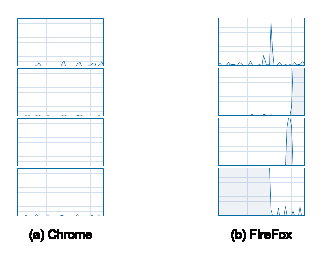
\includegraphics[scale=2]{cpu_browser}
\end{figure}















